\documentclass[a4paper,10pt]{article}

\usepackage{fullpage}%
\usepackage[T1]{fontenc}%
\usepackage[utf8]{inputenc}%
\usepackage[main=francais,english]{babel}%
\usepackage{graphicx}%
\usepackage{url}%
\usepackage{abstract}%
\usepackage{listings}%
\usepackage{tikz}%
\usepackage{amsmath}%
\usepackage{amssymb}%
\usepackage{amsfonts}%
\usepackage{mathtools}%
\usepackage{amsthm}%
\usepackage{array}%
\usepackage{csquotes}%
\usepackage{mathpazo}%
\usepackage{subfig}%
\usepackage[backend=biber]{biblatex}%

\DeclarePairedDelimiter\ceil{\lceil}{\rceil}%
\DeclarePairedDelimiter\floor{\lfloor}{\rfloor}%

\renewcommand\qedsymbol{$\blacksquare$}%

\theoremstyle{definition}

\newtheorem{defi}{Définition}
\newtheorem*{defi*}{Définition}
\newtheorem{theo}{Théorème}
\newtheorem*{theo*}{Théorème}
\newtheorem{exem}{Exemple}
\newtheorem*{exem*}{Exemple}
\newtheorem{prop}{Proposition}
\newtheorem*{prop*}{Proposition}
\newtheorem{coro}{Corollaire}
\newtheorem*{coro*}{Corollaire}
\newtheorem{lemm}{Lemme}
\newtheorem*{lemm*}{Lemme}

\bibliography{papers}% The name of your .bib file

\parskip=0.5\baselineskip

\lstset{%
	basicstyle= \sffamily,%
	columns=fullflexible,%
	frame=lb,%
	frameround=fftf,%
	language=C,%
	numbers=left,%
}%

%
\begin{document}
%
\title{PROG2 : Projet PONG}
%
\author{Tom Bachard\and Guillaume Barbier\and Victor Careil}
%
\date{\today}
%
\maketitle
%
%

\begin{description}
  \item[Classification ACM] D.m
  \item[Mots-clés] Programmation; Java; JavaFX; Programmation événementielle; PONG
\end{description}

%
\begin{abstract}
Le paradigme de programmation événementielle est très souvent utilisé lorsqu'un utilisateur interagit de manière intermittente avec l'application. Grâce à la bibliothèque JavaFX de Java (anciennement Swing), nous mettons au point un moteur de jeu permettant de jouer au très célèbre jeu PONG.
\end{abstract}
%

%
\section{Introduction}
%

  \subsection{PONG}
  	%
	PONG est l'un des premiers jeux vidéos commercialisés. Inventé en 1972 par Nolan Bushnell et Allan Alcorn, ce jeu propose de faire s'affronter tantôt deux joueurs, tantôt un joueur et un ordinateur, dans un match de tennis de table vu du dessus. C'est le premier jeu qui devient populaire, en attestent les 8000 bornes d'arcade vendues par \emph{Atari} l'année de son invention. Un exemple de partie est donné en figure \ref{Pong1}.
	
	Lors d'un affrontement joueur contre joueur, le jeu doit être capable de gérer les déplacements des deux raquettes en même temps, tout en calculant la trajectoire de la balle, afin que cette dernière soit cohérente et permette une bonne expérience de jeu. Pour cela, nous développons notre PONG en Java, en nous servant de la bibliothèque JavaFX (anciennement Swing), spécialisée dans le traitement d'événements interactifs concurrents.
	
	\begin{figure}
  	  \begin{center}
    	    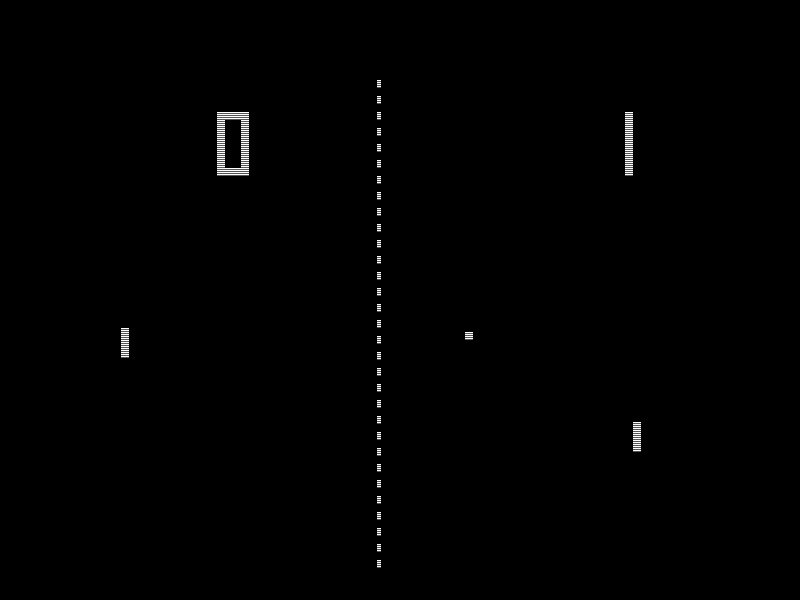
\includegraphics[width=0.5\textwidth]{Pong1}
    	    \caption{Une partie de Pong.}
    	    \label{Pong1}
  	  \end{center}
	\end{figure}	
	
	
  \subsection{Programmation événementielle}
  	%
	La programmation événementielle est un paradigme de programmation qui, par opposition à la programmation séquentielle, s'appuie sur les événements et leur réactions qu'elle reçoit. Ce qu'on définit comme \og événement \fg{} est très large, en effet, sont considérés comme tels les actions suivantes:
	\begin{itemize}
		\item l'ajout d'élément dans une liste ;
		\item le changement d'état d'un booléen ;
		\item le clic d'une souris ;
		\item la pression d'une touche de clavier\dots
	\end{itemize} 
	
	On remarque que ces points, et notamment les deux derniers, sont très intéressants dans la réalisation d'un jeu tel que PONG. En effet, considérer les positions des différentes raquettes, ainsi que la balle, comme des événements permet une implantation simple et élégante de ce jeu.

	De plus, cette notion d'évennement change la façon dont sont gérés les acteurs. Si l'affichage a besoin de la position de la balle, ce n'est pas à la balle de donner sa position à l'affichage, mais c'est plutôt à l'affichage de réagir à l'évènement \og la balle a bougé \fg. Ceci change la logique et l'organisation du code pour le mieux.
	
	Enfin, il est à noté que la programmation événementielle est généralement utilisée avec des langages de haut niveau, ce qui justifie notre utilisation de Java.
	
\section{Concepts généraux}
%

    \subsection{Les \emph{timelines}}
    %
    La principale source d'animation dans notre jeu sera gérée à travers les \emph{timelines}. En effet, cette bibliothèque permet d'animer les représentation graphiques de nos objets. Il suffit, par exemple pour la balle, de calculer son prochain point d'intersection, le temps où elle réalisera la collision, et il n'y a plus qu'à faire avancer la balle selon son vecteur vitesse jusqu'à ce qu'elle arrive au point d'intersection calculé. En prévision du prochain déplacement, on calcule aussi la prochaine direction de déplacement de la balle après le rebond.
    
    \subsection{Utilisation des \emph{bindings}}
    %
    Afin de répondre au mieux au problème posé, nous avons décidé d'utiliser les \emph{bidings} proposé par \lstinline{JavaFX}. En effet, ces derniers permettent de lier nos objets, et surtout leur propriétés, aux événements extérieurs, notamment liés aux joueurs. Sans entrer directement dans les détails, on voit bien que l'on pourra, entre autres, lier la position de la balle à son affichage.
    
    \subsection{Séparation du rendu et des calculs}
    %
    Dans l'optique de rendre notre code solide et modulable, nous appliquerons le principe de \og séparation des deux mondes \fg{}. En effet, le monde des calculs mathématiques, trajectoires, rebonds, \dots, et celui du rendu des figures à l'écran, balle, raquettes, \dots, ne doivent pas se croiser. Les classes graphiques ne doivent rien calculer, cela permet de changer radicalement la manière de calcul sans avoir à toucher à ces classes. On pourra même attester de cette robustesse dans notre code puisqu'après la seconde démonstration, nos collisions ont été entièrement refaites, sans avoir à toucher à quoi que se soit dans nos classes graphiques.

    Nous avons également deux systèmes de coordonnées, un système local o\'u sont effectué les calculs et la logique interne du jeu. Ce système de coordonnées peut ensuite être converti dans un système de coordonnées graphique qui lui est uniquement dédié à l'affichage. Ainsi, la logique interne du jeu Pong n'a pas à dépendre de la bibliothèque JavaFX qui gère l'affichage.
    
\section{Implémentation de notre PONG}
%

Lors de la réalisation du jeu, nous avons séparé les classes en deux catégories, comme expliqué précédemment. D'une part, nos classes de calculs, vivants dans un monde purement mathématique, et d'autre part nos classes graphiques, qui appellent les fonctions des premiers classes afin de dessiner les objets aux bons endroits.

    \subsection{Classes du moteur de jeu}
    %
    Nous avons choisi de créer un petit moteur de jeu lors de ce projet, principalement de rendre les collisions des balles avec les murs ou raquettes. On pourra noter dans le package \emph{core} des énumérations et des interfaces, tant pour la lisibilité du code que pour sa modularité.
    	
	\subsubsection*{Classe \emph{Vector2D}}
	%
	Ce classe contient une classe abstraite de vecteur en deux dimensions, utiles pour tous nos calculs. On y retrouve les fonctions classiques d'addition, multiplication, de norme, mais aussi des plus spécifiques à notre jeu telles que des rotations, de calcul d'un vectur normal, ou d'ajout d'une petite perturbation angulaire aléatoire (utile pour que les parties ne soient pas toutes identiques).
	
	\subsubsection*{Classe \emph{Engine}}
	%
	Le fichier \emph{Engine} est la pièce principale du moteur. En effet, c'est lui qui contient l'entièreté des constantes liées au jeu. De plus, des méthodes classiques aux moteurs de jeu nous permettent de gérer facilement le lancement du jeu, son arrêt, les conditions de victoires, \emph{etc}. C'est aussi cette classe qui gère la scène qui contiendra les objets que l'on générera et déplacera lors du jeu.
	
	De plus nous considérons que certaines valeurs, telles que la position des raquettes, font partie intégrante du jeu. Plutôt que de les reléguer à des classes qui gèrent les raquettes, ces valeurs sont des \og Property \fg qui appartiennent à la classe \emph{Engine}. Ce sera ensuite aux classes filles de \emph{Racket} de modifier ces valeurs selont les actions des joueurs.
        \subsubsection*{Classe \emph{World}}
        %
        Cette classe permet de créer la zone de jeu, dont les bordures de la fenêtre, et d'y ajouter les collisions avec les différents éléments présents dans la zone de jeu. On remarquera que les bordures extérieures ne sont pas les seuls objets capables de générer des collisions. 
        
        \subsubsection*{Classe \emph{Borders}}
        %
        L'unique but de ce classe est de calculer les prochaines intersections de la balle avec les bordures. Ce faisant, on peut directement calculer les \emph{timelines} pour la balle. À chaque nouvelle intersection, on recommence le calcul.
        
        Les collisions sont gérées sur les vitesses selon l'axe des abscisses ou des ordonnées, selon le type de collision.
        
        \subsubsection*{Classe \emph{LevelManager}}
        %
        Notre implémentation de PONG propose, une fois un certain score atteint, de passer d'un niveau à un autre. C'est au travers de cette classe qu'est réalisée la transition des niveaux, avec la fonction \emph{nextLevel}. La structure de sauvegarde des niveaux est invisible pour le reste du programme.
        
        C'est aussi ici que sont gérés les différents textes qui apparaissent au cours du jeu, comme par exemple les scores (dynamiques) et les messages de victoire.
        
    \subsection{Classe de rendu graphique}
    %
    Afin de respecter le paradigme de séparation moteur/graphique, nous avons implanté pour chaque objet à rendre une classe qui ne s'occupe que d'afficher la figure géométrique concernée. Chacun de nos \emph{renderer} est en réalité une extension simple d'une classe Java déjà existante, permettant des modifications simples:
    
    \begin{itemize}
      \item \emph{SimpleRacketRender}, qui affiche les raquettes, étend la classe \emph{Rectangle} ;
      \item \emph{SegmentRender}, qui affiche les segments, étend la classe \emph{Line} ;
      \item \emph{BallRender}, qui affiche la balle, étend la classe \emph{Circle}.
    \end{itemize}
    Dans le code, on ne voit que de rares appels à des fonctions du moteur de jeu, la plupart étant des \emph{bindings}. Cela confirme la séparation des deux univers.
    
    \subsection{Dialogue entre agents}
    %
    
    Compte tenu de ces nombreuses classes et des bindings, de nombreux agents communiquent au cours de l'exécution du programme. On donne en figure \ref{fig:diag} l'ensemble de ces communications, qui sont perçus au travers de nos différentes classes exprimées précédemment.
    	\begin{figure}[!h]
  	  \begin{center}
    	    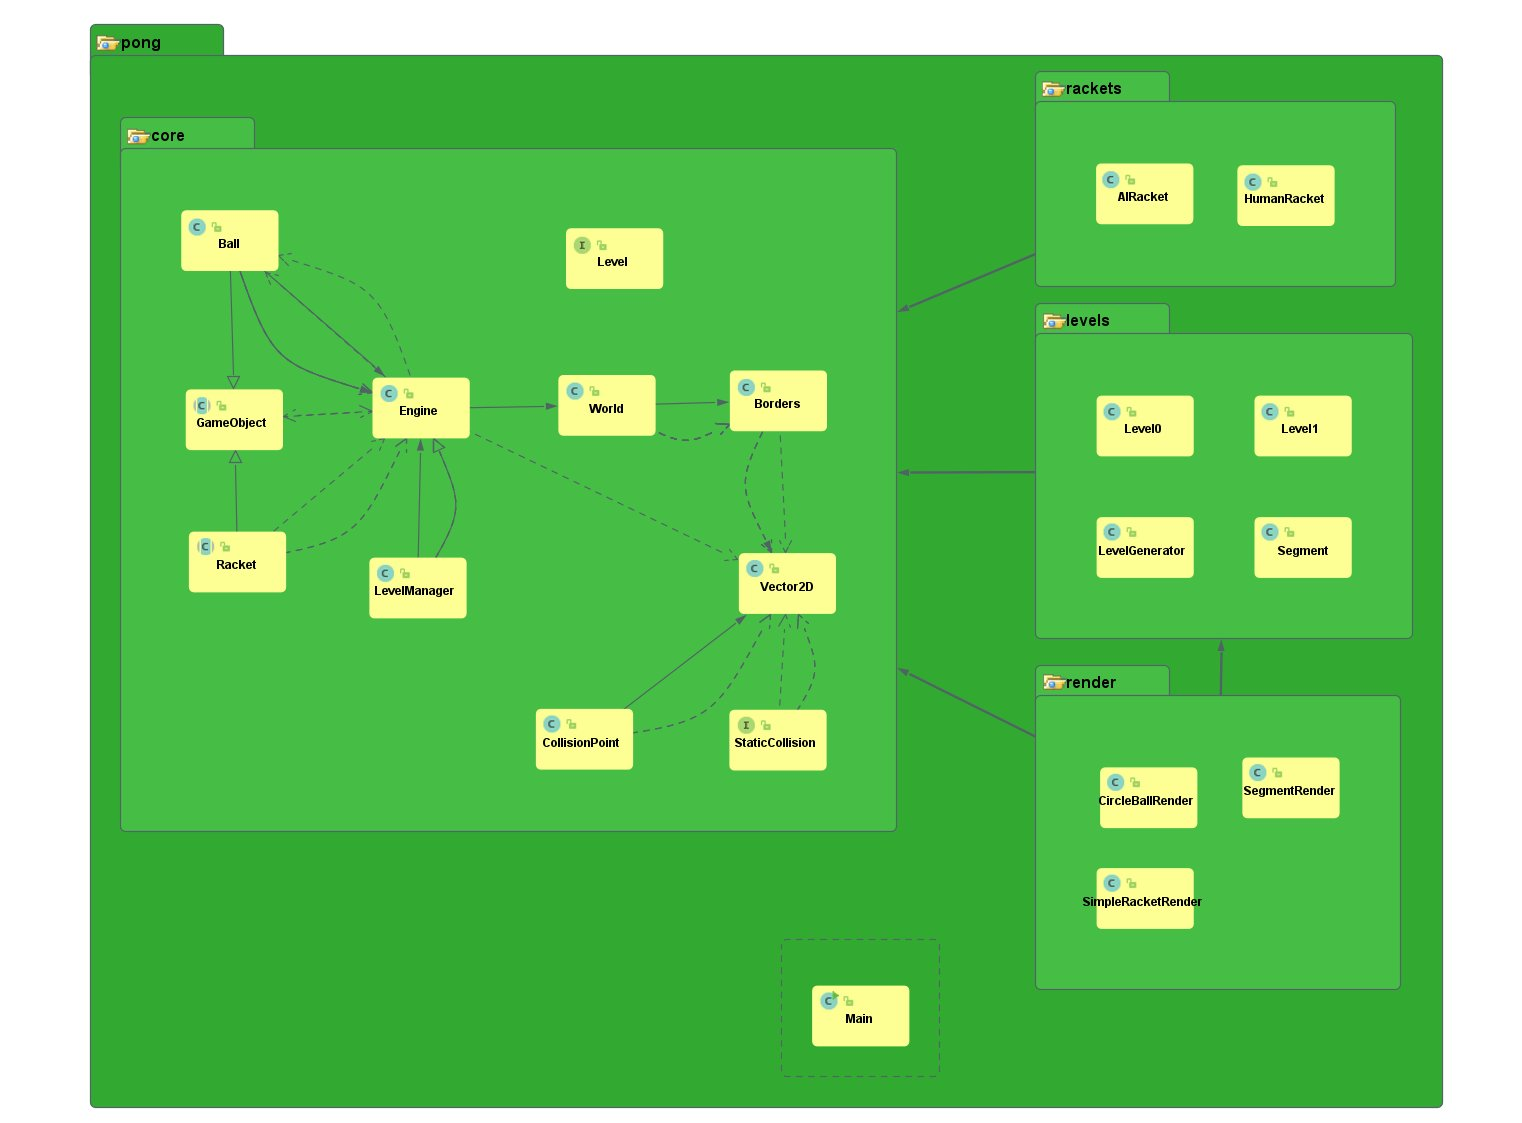
\includegraphics[width=\textwidth]{Class_diagram.jpg}
    	    \caption{Diagramme de classe.}
    	    \label{fig:diag}
  	  \end{center}
	\end{figure}	

\section{Extensions}
	%
	Notre implémentation du jeu PONG propose comme extension la possibilité de jouer à plusieurs niveaux différents. En effet, lorsque l'un des joueurs atteint le score de 5, le niveau actuel change, et les scores sont remis à zéro. La classe \emph{LevelManager} s'occupe de la gestion des niveaux.
	
	De plus, s'ajoute à cette fonctionnalité la possibilité de créer des niveaux nous même. Un créateur de niveaux, au travers de la classe \emph{LevelGenerator}, propose une interface simple, mais \og codée en dur \fg{}, de créer des classes de niveaux, à l'instar de \emph{Level0} et \emph{Level1}, comme le montre la figure \ref{fig:level1}. Actuellement, il est possible de créer des segments, des rectangles et des losanges, mais, il suffit de penser à d'autres formes géométriques à implémenter et à les écrire dans \emph{LevelGenerator} pour améliorer l'interface de création. 
		
	\begin{figure}[!h]
  	  \begin{center}
    	    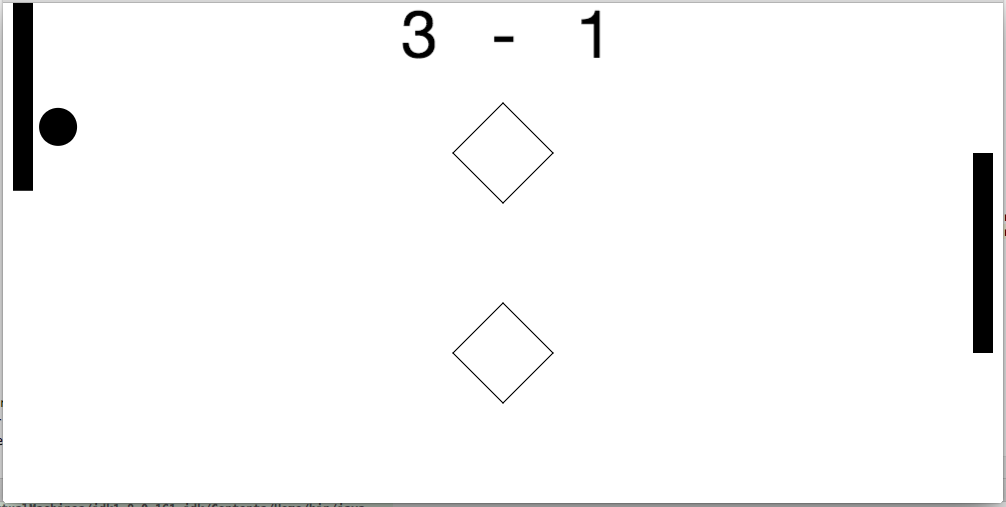
\includegraphics[width=\textwidth]{level1.png}
    	    \caption{Exemple de niveau PONG.}
    	    \label{fig:level1}
  	  \end{center}
	\end{figure}
	
	On remarque aussi que, bien que non réalisée, s'esquisse une implémentation d'un créateur de niveau avec une interface utilisateur.


\end{document}
